\section{Methodik}
\subsection{Softwarearchitektur}
\subsection{Kennzeichenerkennung}
Die Kennzeichenerkennung ist ein Verfahren der Bildverarbeitung, das zur Erkennung und Interpretation von Fahrzeugkennzeichen auf Bildern oder Videoaufnahmen eingesetzt wird. Sie findet Anwendung in zahlreichen Bereichen wie der Verkehrsüberwachung, Mauterfassung, Parkraumbewirtschaftung oder Zufahrtskontrolle.\\\\
Das System basiert im Wesentlichen auf drei zentralen Prozessschritten: der Bilderfassung, der Lokalisation des Kennzeichens im Bild sowie der Texterkennung. Zunächst wird ein Bild eines Fahrzeugs aufgenommen, durch eine Kamera. Im nächsten Schritt wird das Kennzeichen im Bild identifiziert dies geschieht mithilfe moderner Objekterkennungsalgorithmen wie YOLO oder klassischer Verfahren der Konturenerkennung. Nachdem der relevante Bildausschnitt extrahiert wurde, folgt die optische Zeichenerkennung, bei der die alphanumerischen Zeichen des Kennzeichens ausgelesen und digital erfasst werden.\\\\
Die Genauigkeit der Kennzeichenerkennung hängt stark von der Qualität der Vorverarbeitung ab, bei der Methoden wie Graustufenumwandlung, Rauschfilterung, Binarisierung und Kantenanalyse eingesetzt werden, um ein möglichst klares Bild für die Texterkennung zu erzeugen. Moderne Systeme kombinieren dabei klassische Bildverarbeitung mit maschinellem Lernen, um auch bei schwierigen Lichtverhältnissen, verzerrten Perspektiven oder verunreinigten Kennzeichen verlässliche Ergebnisse zu erzielen.

\subsubsection{Systemarchitektur und Funktionsweise}
Das implementierte System zur Kennzeichenerkennung basiert auf einer Kombination aus Hardware- und Softwarekomponenten. Für die grundlegende Funktionsfähigkeit werden folgende Hardware-Voraussetzungen benötigt: ein Raspberry Pi oder ein funktionsfähiger Computer, eine handelsübliche oder integrierte Webcam, eine SD-Karte mit dem entsprechenden Betriebssystem-Image für den Raspberry Pi sowie eine Tastatur, Maus und ein HDMI-Kabel zur Verbindung mit einem Monitor. Alternativ können Tastatur, Maus und HDMI-Kabel entfallen, wenn der Raspberry Pi über den RealVNC Viewer ferngesteuert und eingerichtet wird.\singlespacing 
Auf der Softwareseite kommen verschiedene Technologien zum Einsatz. Zur Objekterkennung wird das Modell YOLOv5 verwendet, während OpenCV zur Bildverarbeitung und Tesseract OCR für die Texterkennung eingesetzt werden. \singlespacing
Der Ablauf der Kennzeichenerkennung erfolgt in drei Schritten: \\
1. Bilderfassung: Die Kamera nimmt acht Bilder auf, die lokal auf dem Gerät gespeichert werden.\\
2. Erkennung: Die gespeicherten Bilder werden mithilfe von YOLOv5 analysiert. Die erkannten Kennzeichenbereiche (Bounding Boxes) werden markiert und die Bilder erneut gespeichert. \\
3. Texterkennung: Im letzten Schritt erfolgt die optische Zeichenerkennung (OCR) mit Tesseract. Dabei werden die Buchstaben extrahiert, separat gespeichert und das erkannte Kennzeichen im Konsolenfenster ausgegeben. \\

Das System wurde speziell am Beispiel für den Einsatz an europäischen Mautstationen konzipiert und optimiert.

\subsubsection{Training und Optimierung des Modells}
Für die Erkennung der Kennzeichenbereiche wurde bewusst das Modell YOLOv5 eingesetzt. Dieses Modell bietet eine ausgewogene Kombination aus Genauigkeit und Effizienz und eignet sich besonders gut für ressourcenbeschränkte Umgebungen wie den Raspberry Pi. Zwar existieren mittlerweile neuere und theoretisch leistungsfähigere Modellversionen, doch diese bringen meist deutlich höhere Anforderungen an Rechenleistung und Speicher mit sich, was eine stabile Ausführung auf einem Mikrocomputer wie dem Raspberry Pi erschwert oder sogar unmöglich macht. Gerade im Hinblick auf die beschränkten Hardwarekapazitäten des Raspberry Pi ist YOLOv5 insbesondere in den Varianten „nano“ oder „small“ eine sinnvolle Wahl. Diese Varianten sind speziell darauf ausgelegt, auch auf schwächerer Hardware zuverlässig zu funktionieren und dabei dennoch eine ausreichend hohe Erkennungsgenauigkeit zu gewährleisten. In der Praxis zeigt sich, dass mit YOLOv5 eine robuste Objekterkennung in nahezu Echtzeit möglich ist, ohne den Systembetrieb zu beeinträchtigen.\\

Zur Detektion von KFZ-Kennzeichen im Bildmaterial kommt in unserem Projekt ein speziell trainiertes YOLOv5-Modell zum Einsatz. YOLO  ist eine auf Echtzeit ausgelegte Objekterkennungsarchitektur, die es ermöglicht, Objekte wie Nummernschilder direkt in Bildern zu lokalisieren und zu klassifizieren. Wir haben uns dabei für die besonders kompakte Variante YOLOv5n (nano) entschieden, da diese für ressourcenschwache Systeme wie den Raspberry Pi 4 optimiert ist und eine hohe Inferenzgeschwindigkeit bei geringer Modellgröße bietet.

\paragraph{Datengrundlage}

Als Trainingsgrundlage diente ein öffentlich zugänglicher Datensatz aus Roboflow Universe mit rund 3.000 annotierten Bilder von KFZ-Kennzeichen. Der Datensatz enthält bereits diverse Perspektiven, Lichtverhältnisse und Rotationen, was zur Robustheit des Modells beiträgt.\\

Zusätzlich wurden während des Trainings verschiedene Datenaugmentierungen vorgenommen, um die Generalisierungsfähigkeit weiter zu verbessern. \cite{roboflowdataset} Hierzu zählten unter anderem:

\begin{itemize}
    \item Auto-Orientierung zur Korrektur der Bildausrichtung
    \item Resize auf ein einheitliches Format von 640x640 Pixel
    \item Rauschüberlagerung (bis zu 1{,}6\% der Pixel)
    \item Unschärfeeffekte (bis zu 1{,}6\% Pixel Blur)
  \end{itemize}

Diese Maßnahmen wurden mit Roboflow automatisiert vorgenommen. Das Modell wurde anschließend in Google Colab auf einer GPU-Instanz trainiert. Die Trainingsdauer betrug etwa 1,5 bis 2 Stunden. Als Hyperparameter wurden 50 Epochen mit einer Batch-Größe von 10 verwendet. Die restlichen Parameter (zum Beispiel Lernrate) blieben auf den Standardwerten des YOLOv5-Frameworks.

\paragraph{Trainingsergebnisse und Validierung}{}

Zur Bewertung des Trainingsverlaufs wurden typische Metriken von YOLOv5 analysiert. Abbildung~\ref{fig:training} zeigt die Entwicklung der Kennzahlen über den Verlauf von 50 Trainings-Epochen.\\

\begin{figure}[h]
    \centering
    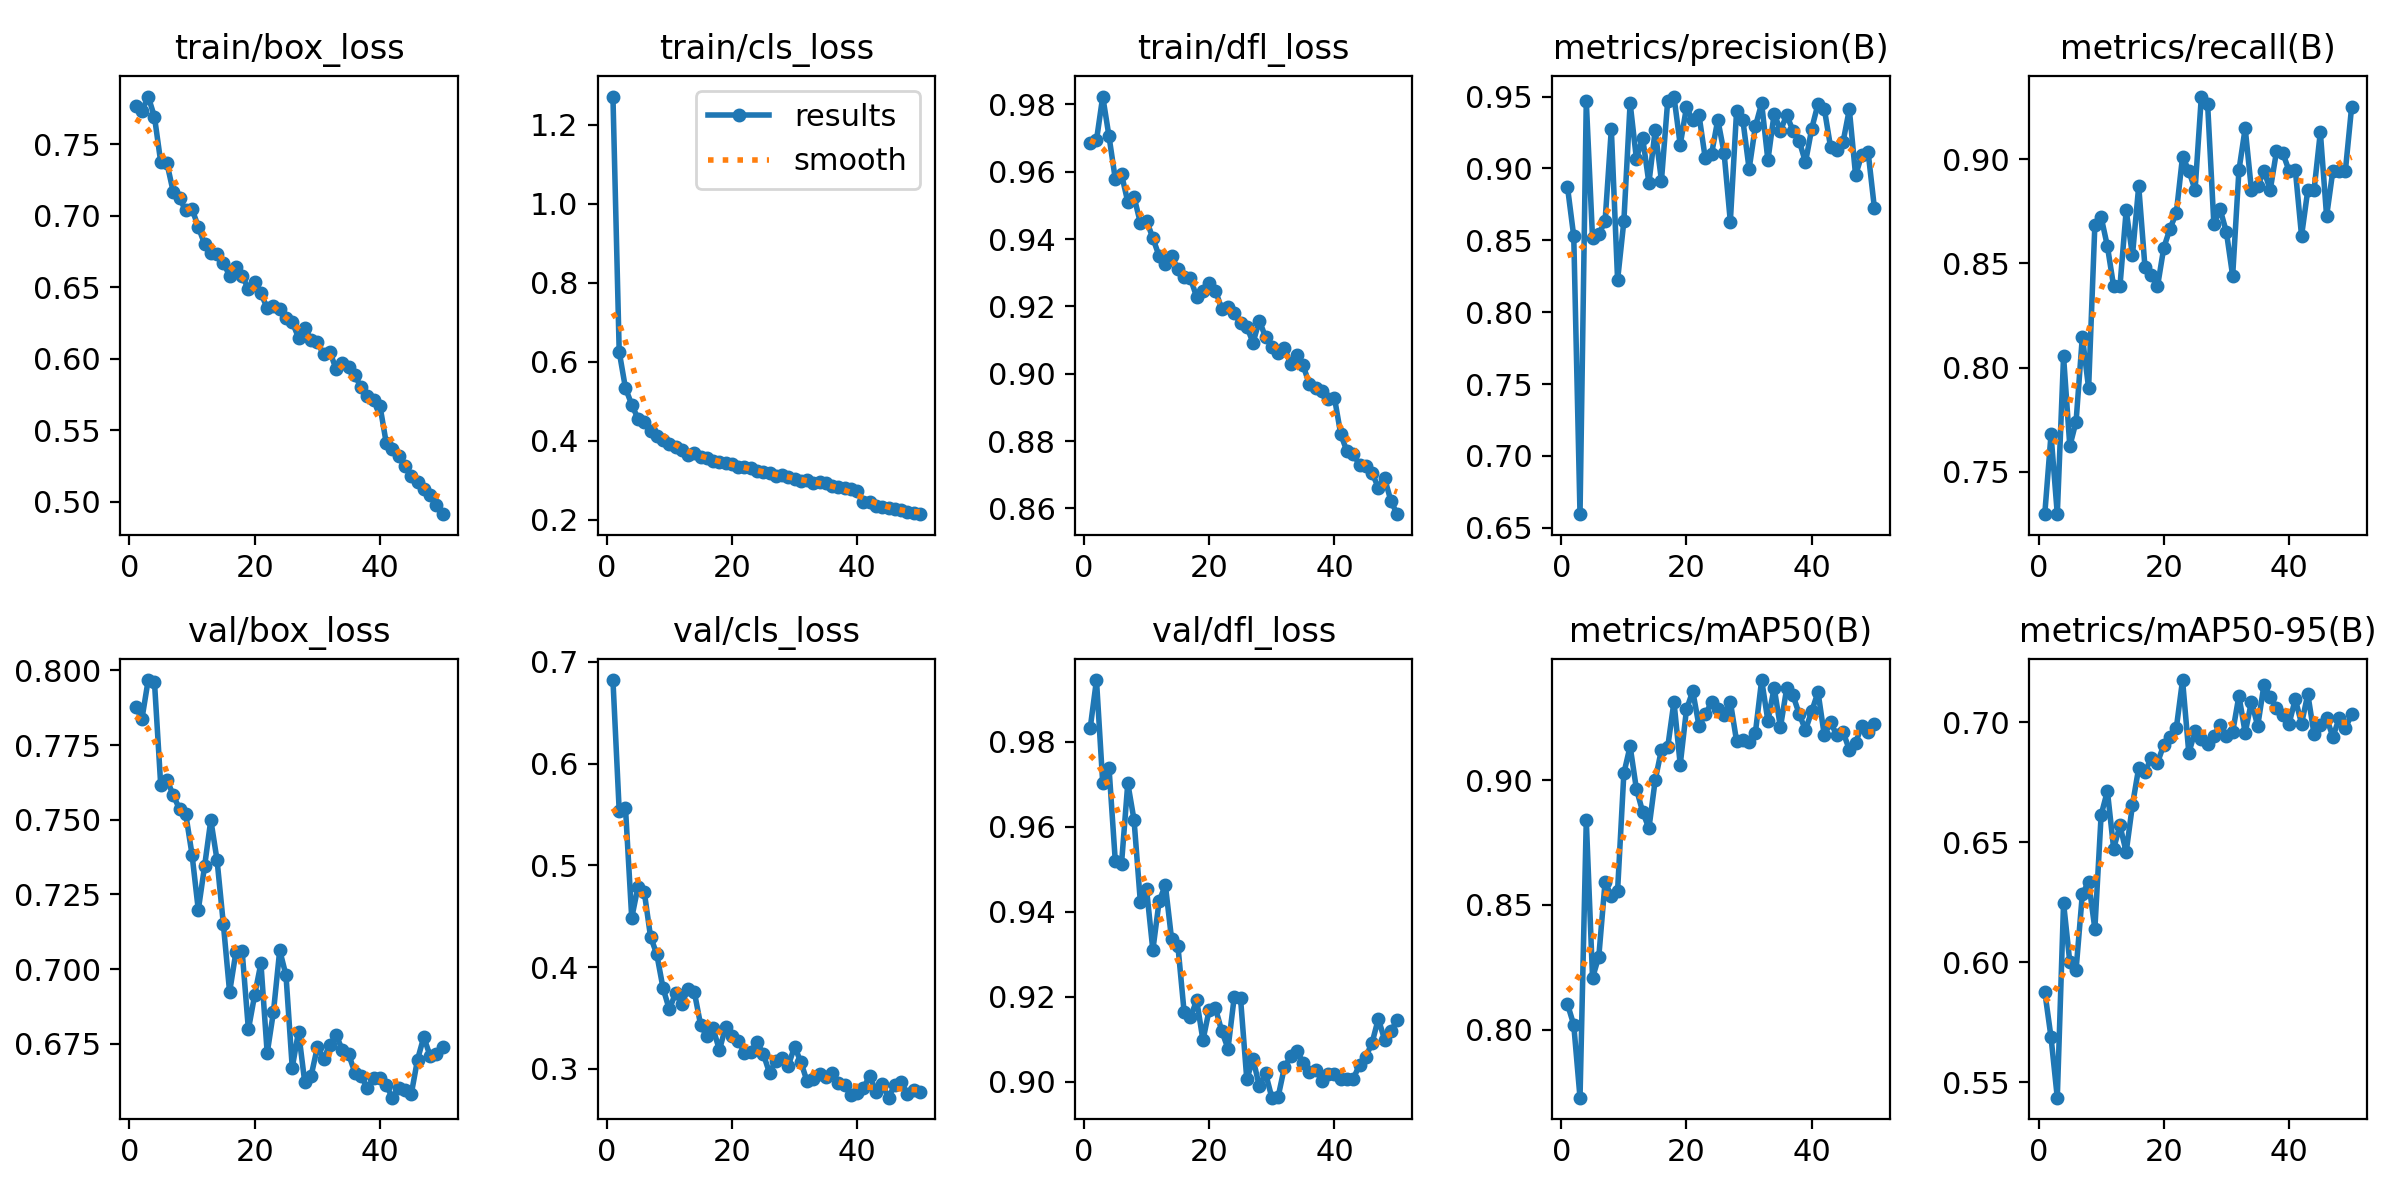
\includegraphics[width=0.55\textwidth]{data/training_results.png}
    \caption{Trainingsergebnisse des YOLOv5-Modells.}
    \label{fig:training}
\end{figure}

Zu erkennen ist, dass sowohl die Trainings- als auch Validierungsverluste (box\_loss, cls\_loss, dfl\_loss) im Verlauf kontinuierlich abnehmen, was auf ein stabiles und erfolgreiches Training hindeutet. Besonders der Klassifikationsverlust (cls\_loss) zeigt eine schnelle Konvergenz in den ersten zehn Epochen. Die Präzision und der Recall pendeln sich im oberen Bereich ein – teils mit leichten Schwankungen, die jedoch durch das kleine Modell und die geringe Batch-Größe erklärbar sind.\singlespacing

Besonders relevant ist der mean Average Precision (mAP) – ein Maß für die Genauigkeit bei verschiedenen IoU-Schwellenwerten. Der Wert mAP@0.5 steigt im Verlauf des Trainings auf über 0,9, während mAP@0.5:0.95 einen stabilen Endwert um 0,70 erreicht. Dies spricht für eine hohe Detektionsqualität, auch bei komplexeren Szenarien.
\paragraph{Konfidenz und Modellanwendung}
Die Ausgabe eines YOLO-Modells enthält neben den erkannten Objektpositionen auch sogenannte Konfidenzwerte, also Wahrscheinlichkeiten, mit denen das Modell ein Objekt als erkannt einstuft. In unserem Projekt wurde ein Konfidenzschwellenwert definiert, um falsch-positive Erkennungen zu reduzieren. Nur Detektionen mit einer Konfidenz über diesem Schwellenwert wurden weiterverarbeitet.\singlespacing

Das trainierte YOLOv5-Modell im .pt-Format wurde zur Performanzoptimierung in das NCNN-Format konvertiert. NCNN ist ein hochoptimiertes Inferenz-Framework speziell für mobile und eingebettete Systeme. Dadurch konnte das Modell auf dem Raspberry Pi 4 mit hoher Effizienz ausgeführt werden. Die Anwendung läuft in einem Skript, das serienweise acht Bilder aufnimmt und analysiert – was nahezu Echtzeitverarbeitung ermöglicht.

\paragraph{Einfluss der Trainingsdaten und Verbesserungsmöglichkeiten}
Die Qualität und Diversität der Trainingsdaten hat direkten Einfluss auf die Erkennungsleistung. In unserem Fall war der Datensatz breit gefächert, jedoch auf Kennzeichen fokussiert. Mögliche Optimierungen für die Zukunft wären:

\begin{itemize}
    \item Erweiterung des Datensatzes um reale eigene Aufnahmen
    \item Feinjustierung der Augmentierungstechniken
    \item Transfer Learning mit größeren Basismodellen
    \item Active Learning durch gezieltes Nachtraining mit fehlerhaften Beispielen
  \end{itemize}

  Dadurch könnte die Robustheit des Modells gezielt für Spezialfälle wie Nachtaufnahmen, verschmutzte Kennzeichen oder ungewöhnliche Kamerawinkel verbessert werden.


\subsubsection{Image Preprocessing}

Die Bildvorverarbeitung dient der Verbesserung der visuellen Eigenschaften der Bildausschnitte, in denen die Nummernschilder enthalten sind. Ziel ist es, die Zeichenstrukturen klar hervorzuheben, Bildrauschen zu minimieren und die Voraussetzungen für eine spätere Weiterverarbeitung, beispielsweise durch Texterkennung, zu schaffen.\singlespacing

Der erste Schritt der Pipeline besteht in der Umwandlung des Originalbildes in ein Graustufenbild. Dieses wird anschließend um den Faktor 3 vergrößert, um relevante Details, insbesondere feine Strukturen von Zeichen, deutlicher hervorzuheben. Im Anschluss erfolgt eine Glättung mittels eines Gaußschen Weichzeichners mit einer Kernelgröße von 3$\times$3, um Bildrauschen zu unterdrücken.

Darauf folgt ein binäres Thresholding mit inversierter Darstellung (\texttt{cv2.THRESH\_BINARY\_INV}). Durch diese Umkehrung erscheinen potenzielle Zeichenbereiche weiß auf schwarzem Hintergrund, was die spätere Konturerkennung erleichtert.\singlespacing

Um benachbarte Strukturen zu verbinden und kleinere Lücken in Zeichenformen zu schließen, wird im nächsten Schritt eine morphologische Dilation durchgeführt. Hierbei wird ein rechteckiges Strukturierungselement der Größe 3$\times$3 verwendet.\singlespacing

Die vorbereiteten Bilder werden im Anschluss zur Konturerkennung verwendet, wobei die Konturen in der Regel einzelnen Zeichen oder Zeichenkomponenten entsprechen. In späteren Verarbeitungsschritten können diese Bereiche gezielt extrahiert und analysiert werden.\singlespacing

Durch diese Kette an Vorverarbeitungsschritten wird sichergestellt, dass relevante Bildinformationen betont und störende Einflüsse reduziert werden, um die Qualität der anschließenden Bildanalyse zu maximieren.


\subsubsection{Optical Character Recognition}

Nach Abschluss der Bildvorverarbeitung, bei der die Kennzeichenbilder in eine geeignete Form gebracht wurden, erfolgt die Erkennung der enthaltenen alphanumerischen Zeichen mittels Optical Character Recognition (OCR). Zu Beginn des Projekts wurden dazu verschiedene OCR-Engines untersucht, darunter auch EasyOCR. Diese Deep-Learning-basierte Bibliothek liefert in vielen Anwendungsfällen gute Ergebnisse, zeigte jedoch im praktischen Einsatz auf ressourcenschwacher Hardware wie dem Raspberry Pi 4 deutliche Einschränkungen. Der hohe Speicherbedarf und die langen Inferenzzeiten verhinderten eine Echtzeitverarbeitung.\singlespacing

Im Vergleich dazu bot Tesseract eine deutlich geringere Systemlast bei gleichzeitig stabiler Erkennungsleistung. Besonders in unserem Anwendungsfall – kontrastreiche, segmentierte Kennzeichenbilder – erwies sich Tesseract als ausreichend genau. Durch gezielte Konfigurationsmöglichkeiten, wie die Beschränkung auf bestimmte Zeichensätze und Layout-Modi, ließ sich die Leistung zusätzlich optimieren. Aus diesen Gründen fiel die Entscheidung auf die Kombination aus Tesseract und der Python-Bibliothek \texttt{pytesseract}.\singlespacing

Im nächsten Schritt der Pipeline erfolgt eine Konturanalyse auf dem vorbereiteten binären Bild. Die erkannten Konturen werden nach verschiedenen geometrischen Kriterien gefiltert, um nur relevante Regionen weiterzuverarbeiten – etwa anhand von Größe, Seitenverhältnis und Position. Für jede verbleibende Kontur wird ein leicht vergrößerter Bildausschnitt (Region of Interest) definiert. Dieser wird an die OCR-Engine übergeben.\singlespacing

Die Texterkennung wird über die Funktion \texttt{image\_to\_data} durchgeführt. Dabei wird der zu analysierende Zeichensatz auf Großbuchstaben und Ziffern eingeschränkt (\texttt{tessedit\_char\_whitelist}) und mit dem Seitenlayout-Modus \texttt{--psm 8} gearbeitet, der für einzelne Zeichen geeignet ist. Das Ergebnis umfasst neben dem erkannten Text auch Positionsdaten und Konfidenzwerte.\singlespacing

Abschließend werden die erkannten Zeichenbereiche im Graustufenbild visuell hervorgehoben und als Bilddateien gespeichert, um die Ergebnisse nachvollziehbar und prüfbar zu machen. \cite{geeksforgeeks2021tesseract}

\subsubsection{Herausforderungen bei realen Bedingungen}
Im Rahmen der Entwicklung unseres Kennzeichenerkennungssystems, das auf eine Mautstationssituation ausgelegt ist, traten verschiedene Herausforderungen auf, die unter realen Bedingungen von besonderer Bedeutung sind. \singlespacing

Eine der ersten Schwierigkeiten bestand in der Vielfalt von Kfz-Kennzeichen weltweit. 
Während die Objekterkennung des Kennzeichens selbst (die Lokalisierung auf dem Bild) zuverlässig funktionierte, erwies sich das anschließende Auslesen der Schriftzeichen als problematisch. 
 Dies lag an den unterschiedlichen Formaten, Schriftarten und Normen, die international variieren. 
 Nach eingehender Analyse kamen wir zu dem Entschluss, dass die Entwicklung eines universellen Kennzeichenerkenners, der alle internationalen Standards abdeckt, den Rahmen unseres Projektes deutlich überschreiten würde. 
 Stattdessen entschieden wir uns, eine optimierte Lösung speziell für deutsche Kfz-Kennzeichen zu entwickeln, um innerhalb der gegebenen Projektgrenzen eine funktional stabile Erkennung zu gewährleisten.\singlespacing
 Eine weitere Herausforderung stellte die Anpassung des Systems an verschiedene Licht- und Schattenbedingungen dar. 
 Schon bei kleinen aber vor allem bei stark wechselnden Beleuchtungsverhältnissen war die Festlegung geeigneter Thresholds bei der Bildverarbeitung für eine universale Lösung herausfordernd. 
 Auch hier zeigte sich, dass eine umfassende allgemeine Lösung, die alle möglichen Umgebungsbedingungen robust abdeckt, einen erheblichen zusätzlichen Entwicklungsaufwand erfordern würde. \singlespacing
 Zudem stießen wir auf technische Grenzen hinsichtlich der Leistungsfähigkeit des eingesetzten Raspberry Pi.
Insbesondere die Schriftzeichenerkennung stellte hohe Anforderungen an die Prozessorleistung, was die Echtzeitfähigkeit des Systems deutlich beeinträchtigte.
Es wurde schnell klar, dass der Raspberry Pi vor allem für den Einsatz unter kontrollierten Laborbedingungen geeignet ist, während für Anwendungen unter realen Bedingungen leistungsstärkere Hardware empfohlen wird.
Die Herausforderung lag hier insbesondere darin, eine akzeptable Balance zwischen Hardwareanforderungen und Systemleistung herzustellen.\singlespacing

Vor diesem Hintergrund entschieden wir uns bewusst für die Verwendung der YOLOv5-Architektur, da diese im Vergleich zu neueren Modellen wie YOLOv8 eine deutlich geringere Rechenlast aufweist und damit besser auf ressourcenbeschränkter Hardware wie dem Raspberry Pi lauffähig ist.
Die Wahl eines leichteren Modells ermöglichte es, die grundlegenden Funktionen der Gesichts- und Schrifterkennung trotz der beschränkten Systemressourcen zuverlässig zu demonstrieren. 
\subsubsection{Optimierung für wechselnde Lichtverhältnisse und Kameraperspektiven}

Zur Verbesserung der Erkennungsstabilität unter realen Bedingungen wird besonderes Augenmerk auf die Bildverarbeitung gelegt. Ein vielversprechender Ansatz besteht in der Nutzung mehrstufiger Preprocessing-Pipelines. Hierbei wird dasselbe Eingangsbild mehreren parallel ausgeführten Vorverarbeitungsschritten unterzogen, die jeweils auf typische Problemquellen wie Überbelichtung, Schatten oder Kontrastarmut optimiert sind. Die resultierenden Varianten werden anschließend bewertet, um die am besten geeignete für die Texterkennung auszuwählen.\singlespacing

Darüber hinaus kann perspektivische Verzerrung durch geometrische Transformationen, etwa mithilfe von Homographie-Matrizen, reduziert werden. Diese Maßnahme ist besonders bei schräg aufgenommenen Kennzeichenbildern sinnvoll, wie sie bei ungünstiger Kameraposition oder ungleichmäßiger Fahrzeugausrichtung entstehen.\singlespacing

Als mögliche Erweiterung wäre ein Postprocessing-Konzept denkbar, bei dem erkannte Zeichenfolgen hinsichtlich ihrer strukturellen Korrektheit überprüft werden. In professionellen Systemen wird dies häufig durch Plausibilitätsprüfungen oder den Vergleich mehrerer Verarbeitungsergebnisse realisiert. Dabei kommen Algorithmen zum Einsatz, die verschiedene OCR-Ergebnisse anhand formaler Merkmale, Zeichensatzvalidität und Konfidenzwerten bewerten, um das wahrscheinlich korrekteste Resultat zu ermitteln. Denkbar wäre zudem der Einsatz eines speziell trainierten KI-Modells, das ausschließlich auf die Erkennung von Schriftarten in KFZ-Kennzeichen ausgelegt ist. Ein solches Modell könnte Unsicherheiten der allgemeinen OCR durch domänenspezifisches Wissen kompensieren und die Gesamterkennungsrate unter realen Bedingungen deutlich verbessern. \cite{marvik2024wild}

\subsubsection{Evaluation und Genauigkeitsanalyse}


\subsection{Gesichtserkennung}
\subsubsection{Testaufbau}
Das implementierte System realisiert eine Echtzeit-Gesichtserkennung mittels einer handelsüblichen Webcam (640$\times$480 Pixel) und verwendet das Modell \texttt{YOLOv8n-face} zur Detektion von Gesichtern. Die Identifikation erfolgt durch Kombination der YOLO-basierten Gesichtserkennung mit dem \texttt{face\_recognition}-Framework, das HOG-basierte Merkmalsextraktion nutzt. Bekannte Gesichter werden im lokalen Verzeichnis gespeichert und können über eine grafische Benutzeroberfläche dynamisch erweitert werden. Das System ist für Zutrittskontrollszenarien konzipiert und erlaubt das Anlernen neuer Gesichter im laufenden Betrieb.

\subsubsection{YOLO}
\paragraph{Vergleich der YOLO-Modelle}
\begin{table}[h]
    \small
    \setlength{\tabcolsep}{6pt} % Weniger Abstand zwischen Spalten
    \renewcommand{\arraystretch}{1.2} % Etwas mehr Zeilenhöhe
    \centering
    \begin{tabular}{|l|c|c|c|c|p{3.8cm}|}
    \hline
    \textbf{Modell} & \textbf{mAP} & \textbf{Zeit (ms)} & \textbf{Parameter} & \textbf{FLOPs} & \textbf{Besonderheiten} \\
    \hline
    YOLOv8n-face   & 39{,}2\%  & 80{,}4  & 3{,}2 Mio. & 8{,}7 Mrd. & Auf Gesichtserkennung spezialisiert \\
    YOLOv8n        & 37{,}3\%  & 80{,}4  & 3{,}2 Mio. & 8{,}7 Mrd. & Generelles Objekterkennungsmodell \\
    YOLOv11n-face* & 41{,}5\%* & 56{,}1  & 2{,}6 Mio. & 6{,}5 Mrd. & Verbesserte Architektur, schneller und effizienter \\
    \hline
    \end{tabular}
    \caption{Vergleich ausgewählter YOLO-Modelle für die Gesichtserkennung. *Werte für YOLOv11n-face geschätzt.}
    \end{table}
    
    \subsection*{Erklärung der Kennzahlen}

\begin{description}
    \item[\textbf{mAP (mean Average Precision)}] 
    Gibt an, wie genau ein Modell Objekte (hier: Gesichter) erkennen kann. Ein höherer mAP-Wert steht für präzisere Lokalisierung und Klassifikation. Bei kleinen Modellen gelten Werte ab etwa 40\,\% als solide.
    
    \item[\textbf{Inferenzzeit (ms)}] 
    Die durchschnittliche Zeit, die das Modell benötigt, um ein einzelnes Bild zu verarbeiten (Vorwärtsdurchlauf). Kürzere Zeiten sind wichtig für Echtzeitanwendungen, z.\,B. bei Live-Video-Streams.
    
    \item[\textbf{Parameter}] 
    Anzahl der im Modell gespeicherten Gewichtungen. Weniger Parameter bedeuten meist geringeren Speicherbedarf und schnellere Verarbeitung, können aber auch die Genauigkeit beeinflussen.
    
    \item[\textbf{FLOPs (Floating Point Operations)}] 
    Maß für den Rechenaufwand pro Bild. Modelle mit niedrigeren FLOPs sind effizienter und benötigen weniger Rechenleistung – ein Vorteil bei Einsatz auf Geräten mit begrenzten Ressourcen.
\end{description}

    Das auf Gesichter spezialisierte Modell YOLOv8n-face erzielt eine höhere Genauigkeit als das generische YOLOv8n. Das neuere YOLOv11n-face bietet voraussichtlich noch bessere Erkennungsraten und eine deutlich schnellere Inferenz, erfordert jedoch ggf. Anpassungen und erneutes Training für die Kompatibilität mit dem aktuellen Code. Generische Modelle wie YOLOv8n erkennen mehr Objekttypen, sind aber für die reine Gesichtserkennung weniger effizient.


\subsubsection{MediaPipe}
\paragraph{Gesichtspunkterkennung: Code} 

Für die Gesichtspunkterkennung nutzen wir das FaceMesh Modell von Mediapipe, das 468 3D-Gesichtspunkte in Echtzeit erfasst. Diese dreidimensionalen Koordinaten ermöglichen vielfältige Anwendungen in Gesichtserkennung, Emotionsanalyse und Augmented Reality.

Der vollständige Code, der die hier beschriebene Gesichtspunkt-Erkennung mit MediaPipe implementiert, ist auf GitHub\cite{github_yolo} verfügbar.
Der ganze Code ist in Python geschrieben.

Zunächst müssen wir notwendigen die Bibliotheken importieren. Diese sind in unserem Fall die OpenCV und MediaPipe-Bibliotheken.
Danach initialisieren wir die MediaPipe-Instanz. Dies geschieht mit dem folgenden Code:
\begin{lstlisting}
    # MediaPipe FaceMesh Setup
    mp_face_mesh = mp.solutions.face_mesh
    face_mesh = mp_face_mesh.FaceMesh(static_image_mode=False, max_num_faces=5, min_detection_confidence=0.8)
\end{lstlisting}

\textbf{Parameter-Erläuterung:}
\begin{itemize}
    \item \texttt{static\_image\_mode=False}: Entscheidend für die Verarbeitung von Videostreams und Live-Kameraaufnahmen, signalisiert dem Modell eine Bildsequenz.
    \item \texttt{max\_num\_faces=5}: Begrenzt die Erkennung auf maximal 5 Gesichter gleichzeitig.
    \item \texttt{min\_detection\_confidence=0.8}: Setzt die Erkennungsschwelle auf 80\% für präzise Resultate bei guter Balance zwischen Genauigkeit und Robustheit.
\end{itemize}

Um die erkannten Gesichtspunkte und deren Verbindungen visuell darzustellen, initialisieren wir die Zeichenwerkzeuge von MediaPipe. \texttt{drawing\_spec} definiert das Aussehen der Punkte und Linien (z.B. Farbe, Dicke).

Im nächsten Schritt wird die Webcam geöffnet, um Videobilder aufzunehmen. Alternativ könnte man hier auch den Pfad zu einer Bild- oder Videodatei angeben. 

Die Hauptschleife des Programms läuft, solange die Kamera aktiv ist. In jeder Iteration der Schleife wird ein neues Bild von der Webcam erfasst und verarbeitet.

Ein wichtiger Schritt ist die Konvertierung des Farbraums des aufgenommenen Bildes von BGR (Blue, Green, Red), dem Standardformat von OpenCV, nach RGB (Red, Green, Blue), das von MediaPipe erwartet wird.
\begin{lstlisting}
    rgb_frame = cv2.cvtColor(frame, cv2.COLOR_BGR2RGB)
\end{lstlisting}
Diese Konvertierung ist notwendig, da unterschiedliche Bibliotheken und Modelle intern mit verschiedenen Farbreihenfolgen arbeiten. Die Verwendung der falschen Reihenfolge kann zu fehlerhaften Ergebnissen führen.

Nun verarbeitet MediaPipe das in RGB konvertierte Bild, um Gesichter zu erkennen und die entsprechenden Gesichtspunkte zu lokalisieren.

Sobald ein oder mehrere Gesichter im Bild erkannt wurden, zeichnen wir die 468 Gesichtspunkte und die Verbindungen zwischen ihnen auf das ursprüngliche Farbbild.
\begin{lstlisting}
    if results.multi_face_landmarks:
    for face_landmarks in results.multi_face_landmarks:
        # draw all landmarks
        mp_drawing.draw_landmarks(
            image=frame,
            landmark_list=face_landmarks,
            connections=mp_face_mesh.FACEMESH_TESSELATION,
            landmark_drawing_spec=drawing_spec,
            connection_drawing_spec=drawing_spec
        )
\end{lstlisting}
\textbf{Parameter-Erläuterung}:
\begin{itemize}
    \item \texttt{image=frame}: Das Originalbild (im BGR-Format) für die Visualisierung der Landmarken.
    \item \texttt{landmark\_list=face\_landmarks}: Die Liste der erkannten Gesichtspunkte für ein einzelnes Gesicht.
    \item \texttt{connections=mp\_face\_mesh.FACEMESH\_TESSELATION}: Die vordefinierten Verbindungen zwischen den Gesichtspunkten, die das FaceMesh Modell verwendet (z.B. um Augenbrauen, Lippen, Gesichtskonturen darzustellen).
    \item \texttt{landmark\_drawing\_spec=drawing\_spec}: Die zuvor definierten Zeichenstil-Spezifikationen für die einzelnen Punkte.
    \item \texttt{connection\_drawing\_spec=drawing\_spec}: Die zuvor definierten Zeichenstil-Spezifikationen für die Verbindungslinien.
\end{itemize}

Schließlich wird das mit den eingezeichneten Gesichtspunkten versehene Bild angezeigt. Die Schleife wird beendet und die Webcam freigegeben, sobald der Benutzer die ESC-Taste drückt oder das Programm manuell beendet.

Dieser Code bildet die Grundlage für unsere Gesichtswiedererkennung.

\paragraph{Gesichtswiedererkennung mit Gesichtspunkten: Code} 

Unser System zur Echtzeit-Gesichtserkennung nutzt MediaPipe FaceMesh, um Gesichter in Videostreams präzise zu erkennen.
Seine Funktionalität umfasst das Erlernen und Speichern neuer Gesichter, das Wiedererkennen bekannter Personen und die Fähigkeit zum kontinuierlichen Dazulernen, wodurch sich die Erkennungsleistung stetig verbessert.

Im Kern unseres Programms steht die Initialisierung, in der das MediaPipe FaceMesh-Modul eingerichtet und die Kamera gestartet wird, wie es in Abschnitt 4.3.3.1 beschrieben ist.
Zudem werden Speicherstrukturen für die Namen bekannter Gesichter und deren charakteristische Gesichtspunkte (Landmarks) vorbereitet.

Die eigentliche Gesichtserkennung erfolgt durch die Funktion \texttt{extract\_face\_landmarks}. Diese nutzt MediaPipe, um detaillierte Gesichtsmerkmale zu extrahieren, wobei ein besonderer Fokus auf 50 Schlüsselpunkte in den Bereichen Augen, Nase, Mund und Augenbrauen liegt.
Um eine konsistente Erkennung zu gewährleisten, werden die Koordinaten dieser Punkte normalisiert. Das heißt, dass sie relativ zur Gesichtsgröße und -position skaliert werden, um Verzerrungen durch unterschiedliche Perspektiven und Entfernungen zu minimieren.
\begin{lstlisting}
    # Define indices for key landmarks (eyes, nose, mouth, etc.)
    key_landmarks_indices = [33, 133, 160, 158, 153, ...] 
    ...
    # Save x, y (normalized coordinates)
    landmarks_array.extend([landmark.x, landmark.y]) 
\end{lstlisting}

Für den Gesichtsvergleich kommt die Methode \texttt{detect\_and\_recognize\_faces} zum Einsatz. Sie vergleicht neu erkannte Gesichtsmerkmale mit den gespeicherten Daten.
Dabei werden gewichtete Abstände zwischen den Punkten berechnet, wobei einzelnen Gesichtsregionen, insbesondere den Augen höhere Bedeutung zugewiesen wird, was die Genauigkeit der Erkennung erhöht.

Unser Programm lernt kontinuierlich neue Gesichtsvarianten, um robuster zu werden. Neue Landmark-Daten werden gespeichert, wenn die Erkennung eine Übereinstimmung zwischen 60\% und 95\% aufweist. 
Bei einer geringeren Sicherheit von 40\% bis 60\% erfolgt das Lernen nur mit einer Wahrscheinlichkeit von 30\%, um falsche Zuordnungen zu vermeiden.
\begin{lstlisting}
    # Continuous learning: Improved strategy for continuous learning
            # Only learn when recognition is relatively certain, but not perfect
            if is_known_face:
                # Low confidence: Try to learn
                if 0.6 < confidence < 0.95:
                    self.add_landmark_to_person(name, landmarks)
                # Very low confidence: Only learn occasionally (reduces false associations)
                elif 0.4 < confidence <= 0.6:
                    # Only learn in 30% of cases to reduce errors
                    if np.random.random() < 0.3:
                        self.add_landmark_to_person(name, landmarks)
\end{lstlisting}

Der Lernprozess unseres Programms ist zweigeteilt. Zum einen können Benutzer aktiv ein neues Gesicht speichern, indem sie auf einen "Learn Face"-Button klicken oder eine bestimmte Taste drücken.
Zum anderen verfügt unser Programm über ein kontinuierliches Lernen. Dabei ergänzt es automatisch neue Gesichtsdaten, sofern diese genügend unterschiedlich zu bestehenden Samples sind.
Eine Diversitätsprüfung stellt sicher, dass keine redundanten Daten gespeichert werden. Dazu wird der Abstand des neuen Landmark-Sets zu allen vorhandenen Sets berechnet, und nur bei ausreichender Unterschiedlichkeit erfolgt die Speicherung.

Während der Laufzeit verarbeitet die Hauptschleife des Programms kontinuierlich neue Bilder der Kamera. Gesichter werden erkannt, Landmark-Daten extrahiert, mit bekannten Gesichtern verglichen, Ergebnisse wie Name und Konfidenzwert angezeigt und Benutzereingaben verarbeitet.

Besondere Features unseres Programms tragen wesentlich zur hohen Leistungsfähigkeit bei:
\begin{itemize}
    \item Gewichtete Erkennung steigert die Genauigkeit.
    \item Kontinuierliches Lernen verbessert die Erkennung über die Zeit
    \item Diversitätsprüfung verhindert das Speichern ähnlicher Gesichtsausdrücke.
    \item Konsistenzprüfung über mehrere Frames verringert Fehlerkennungen.
\end{itemize}

Das Benutzerinterface ermöglicht eine einfache Interaktion.
Erkannte Gesichter werden mit Name und Konfidenzwert angezeigt, und neue Gesichter können bequem gelernt werden.

Die Gesichtsmerkmale werden lokal gespeichert, wobei Pickle zur Serialisierung genutzt wird. Dadurch werden bekannte Gesichter beim nächsten Start automatisch wieder geladen.

Insgesamt entsteht so ein System, das nicht nur Gesichter wiedererkennt, sondern sich auch fortlaufend verbessert und flexibel an neue Gegebenheiten anpasst.

\paragraph{Metriken}
Für die Bewertung der Gesichtspunkterkennung mit MediaPipe haben wir folgende Metriken genutzt, da wird diese am Ende auch noch mit YOLO vergleichen möchten:
\begin{itemize}
    \item \textbf{Confidence Score:} Wahrscheinlichkeit, dass ein Gesicht erkannt wurde.
    \item \textbf{FPS / Inferenzzeit:} Anzahl der Bilder pro Sekunde (FPS) bzw. durchschnittliche Latenz pro Bild.
\end{itemize}

\subparagraph{Confidence Score} 

Um die Zuverlässigkeit der Gesichtserkennung zu bewerten, haben wir die Confidence Scores der MediaPipe-Gesichtserkennung und des FaceMesh Modells analysiert.

In Abbildung \ref{fig:confidence_score_mediapipe} sind die Confidence Scores der Gesichtserkennung (x-Achse) und des FaceMesh Modells (y-Achse) dargestellt. Die blauen Punkte repräsentieren die Gesichter die sowohl erkannt als auch mit dem FaceMesh Modell erkannt wurden. 
Die roten Kreuze zeigen Gesichter, die nur erkannt wurden, aber nicht mit dem FaceMesh Modell erkannt werden konnten.

\begin{figure}[ht]
    \centering
    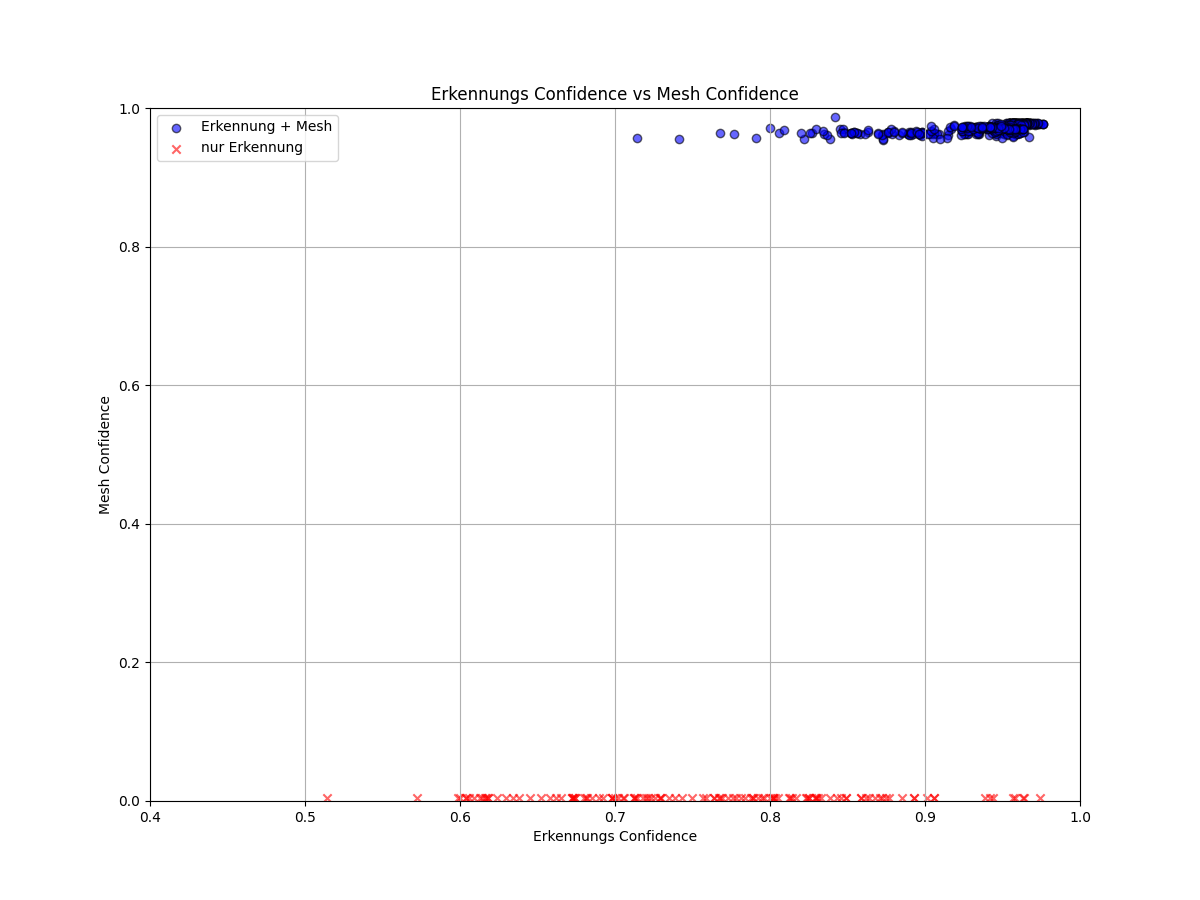
\includegraphics[width=0.55\textwidth]{data/Detection_vs_Mesh_Confidence.png}
    \caption{Confidence Score der Erkennung und FaceMesh}
    \label{fig:confidence_score_mediapipe}
\end{figure}

Obwohl beide Modelle tendenziell hohe Sicherheit in ihren Erkennungen aufweisen (> 0.95), ist die reine Gesichtserkennung deutlich robuster. Wir beobachten wiederholt Fälle, in denen das Detection-Modell hohe Confidence-Werte liefert (z.B. > 0.95), während die zugehörige FaceMesh-Erkennung entweder scheitert oder deutlich niedrigere Scores erzielt.

Die Ursache hierfür liegt in den zusätzlichen Anforderungen der FaceMesh-Erkennung. Sie ist stärker von idealen Aufnahmebedingungen abhängig. Das Gesicht muss vollständig sichtbar sein, die Perspektive geeignet, und die Bildqualität muss detaillierte Analysen erlauben. 
Störungen wie Verdeckungen oder Bewegungen beeinträchtigen die Mesh-Erkennung stärker als die reine Detektion. Zusammenfassend lässt sich festhalten, dass die Gesichtserkennung eine hohe Treffsicherheit besitzt, die Präzision der FaceMesh-Erkennung jedoch maßgeblich von der Qualität der Gesichtsinformationen im Bild beeinflusst wird.

\subparagraph{FPS / Inferenzzeit} 

Die Aufgabenstellung umfasste die Analyse und Bewertung der MediaPipe-Gesichtserkennung und -wiedererkennung hinsichtlich Inferenzgeschwindigkeit, Verarbeitungszeit und Stabilität.

Für die Gesichtserkennung wurden FPS, Verarbeitungszeit und Stabilität bei Confidence-Werten von 50\% und 80\% gemessen und verglichen. Die Gesichtserkennung erfolgte mit MediaPipe FaceMesh auf einer Webcam-Auflösung von 640×480 Pixeln über 60 Sekunden, wobei alle 5 Sekunden Messwerte erfasst wurden.

\begin{figure}
[ht]
    \centering
    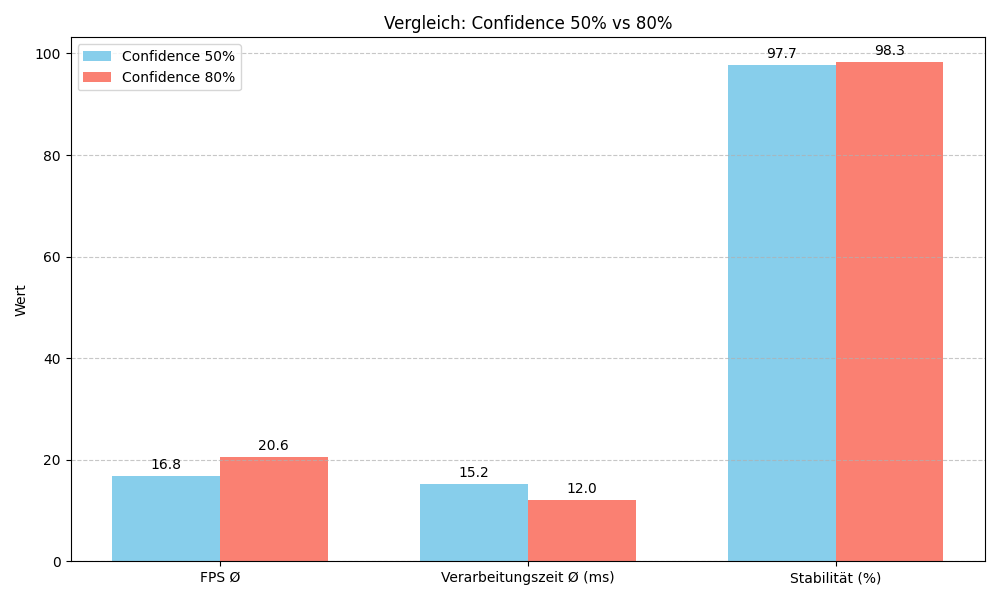
\includegraphics[width=0.55\textwidth]{data/Vergleich_Confidence_50_vs_80.png}
    \caption{Performance bei 50\% vs. 80\% Confidence}
    \label{fig:vergleich_confidence}
\end{figure}

Die Ergebnisse (siehe Abbildung \ref{fig:vergleich_confidence}) zeigen:
\begin{itemize}
    \item Die durchschnittliche Bildrate (FPS) steigt bei einem zunehmenden Confidence-Wert von 50\% auf 80\% von 16,83 FPS auf 219,48 FPS.
    \item Die durchschnittliche Verarbeitungszeit pro Frame sinkt bei einer Erhöhung des Confidence-Werts von 50\% auf 80\% von 15,18 ms auf 12,02 ms.
    \item Die Stabilität der Erkennung steigt leicht an, von 98,64\% bei 50\% auf 99,23\% bei 80\% Confidence.
\end{itemize}
Somit kann man festhalten, dass die Erhöhung des Confidence-Werts von 50\% auf 80\% zu einer signifikanten Verbesserung der Inferenzgeschwindigkeit führt. Ursache dafür ist, dass bei höherer Confidence weniger unsichere Erkennungen verarbeitet werden müssen.

Der FPS-Verlauf über die Zeit (Abbildung \ref{fig:fps_ueber_zeit}) bestätigt diese Tendenz, zeigt aber auch natürliche Schwankungen aufgrund variierender Bildinhalte (z.B. Bewegungen oder Mimik).

Zusammengefasst führt ein höherer Confidence-Wert zu einer schnelleren und stabileren Erkennung, birgt jedoch das Risiko, dass echte Gesichter unter schwierigen Bedingungen übersehen werden. Die Wahl des optimalen Confidence-Werts stellt somit einen Kompromiss zwischen Geschwindigkeit und Erkennungsempfindlichkeit dar.

\begin{figure}[ht]
    \centering
    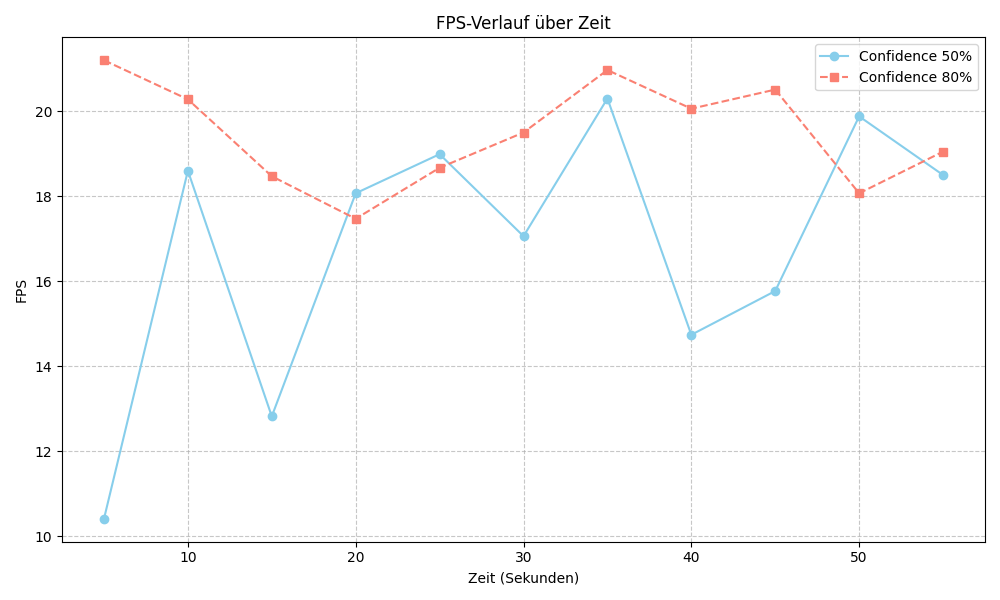
\includegraphics[width=0.55\textwidth]{data/FPS_ueber_Zeit.png}
    \caption{FPS-Werte über Zeitspanne von 60 Sekunden.}
    \label{fig:fps_ueber_zeit}
\end{figure}

Im Anschluss an die Analyse der reinen Gesichtserkennung mit MediaPipe FaceMesh wurde die Performance des erweiterten Systems zur Wiedererkennung gemessen und ausgewertet.

Die Ergebnisse sind in Abbildung \ref{fig:fps_recognition_mediapipe} dargestellt.

Die wichtigsten Ergebnisse sind:
\begin{itemize}
    \item Die durchschnittliche Bildrate (FPS) lag bei 23,55 FPS, womit eine flüssige Echtzeiterkennung gewährleistet ist.
    \item Die Verarbeitungszeit pro Frame betrug im Schnitt 22,71 ms, was eine solide Reaktionsgeschwindigkeit ermöglicht.
    \item Die Stabilität lag im Mittel bei 98,64\%, was auf eine gleichmäßige und zuverlässige Verarbeitung hinweist.
\end{itemize}

\begin{figure}[ht]
    \centering
    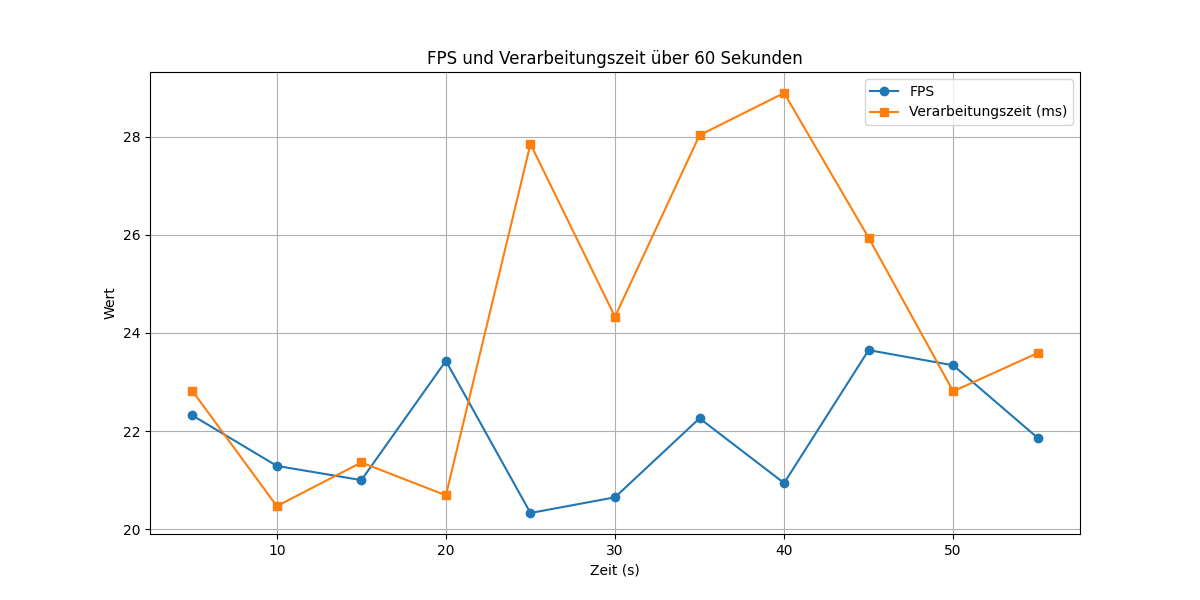
\includegraphics[width=0.55\textwidth]{data/FPS_and_Processing_Time.png}
    \caption{FPS und Verarbeitungszeit bei Wiedererkennung.}
    \label{fig:fps_recognition_mediapipe}
\end{figure}

Verglichen mit der reinen Gesichtserkennung zeigt sich, dass die Integration der Wiedererkennungslogik (Vergleich von Landmark-Distanzen) zwar die durchschnittliche Verarbeitungsgeschwindigkeit leicht reduziert, jedoch weiterhin ausreichend Echtzeitfähigkeit und hohe Stabilität gewährleistet. 
Während bei der reinen Erkennung eine Erhöhung des Confidence-Werts zu einer Steigerung der Geschwindigkeit führte, hängt die Performance der Wiedererkennung primär von der Effizienz der Landmarkverarbeitung und der Distanzberechnung ab.

Unser Programm zeigt eine für viele praktische Anwendungen ausreichende Performance. Die Gesichtserkennung und -wiedererkennung mit MediaPipe FaceMesh kann bei moderater Rechenlast stabil und in Echtzeit arbeiten. 


\paragraph{Anwendungsbeispiel: Zutrittskontrollen}

Mediapipe bietet zwar grundlegende Funktionen zur Gesichtserkennung, weist jedoch erhebliche Einschränkungen bei der zuverlässigen Wiedererkennung von Personen auf. 
Während unser System Gesichter erkennen und deren Merkmale (Landmarks) identifizieren kann, ist es primär für die Erkennung der Gesichtsstruktur konzipiert und nicht für die biometrische Identifikation.

Ein wesentliches Problem ist die langsame Anpassungsfähigkeit. Bei schnellen Bewegungen kann unser System die Wiedererkennung verlieren, wodurch Nutzer gezwungen sind, eine Position zu finden, in der sie erneut erkannt werden. 
Die verwendete Landmark-Distanz-Methode erweist sich als besonders empfindlich: Veränderungen im Gesichtsausdruck, bei Lichtverhältnissen oder der Perspektive können die Lage der Gesichtspunkte signifikant beeinflussen und damit die Wiedererkennung erschweren.

Zudem fehlen wichtige Sicherheitsfunktionen. Es gibt keinen Schutz gegen einfache Täuschungsversuche, beispielsweise könnte jemand ein Foto hochhalten und das System würde dies als echtes Gesicht erkennen. 
Dies macht die Technologie deutlich weniger robust als moderne Face-Recognition-Methoden. Auch die Verwaltung mehrerer Nutzerprofile würde bei diesem einfachen Ansatz schnell komplex und fehleranfällig werden.

Mediapipe wurde eigentlich für andere Anwendungsbereiche entwickelt, insbesondere für Augmented Reality-Anwendungen, bei denen es darum geht, virtuelle Elemente auf Gesichter zu projizieren. 
Seine Stärke liegt in der präzisen Erkennung von Gesichtspunkten, nicht in der Identifikation bestimmter Personen.

Für eine zuverlässige Zutrittskontrolle wären zusätzliche Komponenten erforderlich:
\begin{itemize}
    \item Ein Vergleichssystem mit Face Embeddings und Klassifikationsalgorithmen
    \item Lebenderkennung, um Angriffe mit Fotos oder Videos zu verhindern
    \item Ein zuverlässiges Management-System für gespeicherte Nutzerprofile
\end{itemize}

Zusammenfassend kann Mediapipe durchaus als Baustein für einfache Zugangskontrollen in nicht-kritischen Bereichen dienen (etwa für private Projekte), ist jedoch für sicherheitsrelevante Anwendungen ohne erhebliche Erweiterungen und Kombinationen mit anderen Technologien nicht geeignet. 
Die Stärken des Systems liegen eindeutig in der grundlegenden Gesichtserkennung, während für die zuverlässige Wiedererkennung und Identifikation von Personen fortgeschrittenere Lösungen notwendig sind.

\subsubsection{Vergleich von YOLO und MediaPipe}
\paragraph{Confidence Score}
\paragraph{FPS / Inference Time}

In der durchgeführten Untersuchung zur Gesichtserkennung wurden die beiden Ansätze YOLOv8-face und MediaPipe hinsichtlich ihrer Geschwindigkeit (FPS – Frames per Second) und Stabilität verglichen.
Die Ergebnisse sind in Abbildung \ref{fig:fps_comparison} zusammengefasst.

YOLOv8-face erreicht eine durchschnittliche Bildverarbeitungsrate von etwa 5 bis 6 FPS. Die Stabilität der Gesichtserkennung liegt zwischen 90\% und 99\%, schwankt jedoch stärker im Vergleich zu MediaPipe.
MediaPipe zeigt eine deutlich höhere Bildverarbeitungsrate mit durchschnittlich 20 bis 22 FPS. Die Stabilität bleibt konstant auf einem sehr hohen Niveau zwischen 97\% und 99\%.

Die Ergebnisse zeigen, dass MediaPipe wesentlich schneller arbeitet als YOLOv8-face. Ein höherer FPS-Wert bedeutet, dass MediaPipe mehr Bilder pro Sekunde verarbeiten kann, was für Anwendungen mit Echtzeitanforderungen, wie etwa Videokonferenzen oder mobile Gesichtserkennung, entscheidend ist.
Bezüglich der Stabilität sind beide Systeme sehr zuverlässig. MediaPipe zeigt jedoch eine gleichmäßigere Leistung, während YOLOv8-face gelegentlich größere Schwankungen aufweist.

Die Unterschiede lassen sich auf die jeweilige Architektur der Systeme zurückführen. YOLOv8 basiert auf tiefen neuronalen Netzen und benötigt dadurch mehr Rechenleistung, bietet jedoch eine hohe Genauigkeit und Flexibilität, insbesondere in komplexeren Erkennungsszenarien. 
MediaPipe hingegen verwendet hochoptimierte Algorithmen, die speziell für Echtzeitanwendungen auf mobilen oder ressourcenschwächeren Geräten entwickelt wurden. Dadurch kann MediaPipe eine hohe Geschwindigkeit bei gleichzeitig hoher Erkennungsstabilität erreichen.

Für Echtzeitanwendungen, bei denen Geschwindigkeit und konstante Erkennungsqualität im Vordergrund stehen, ist MediaPipe die bessere Wahl. 
Wenn jedoch die Genauigkeit oder Flexibilität der Erkennung wichtiger ist und eine leistungsstarke Hardware zur Verfügung steht, kann YOLOv8-face von Vorteil sein.

\begin{figure}
    \centering
    \begin{subfigure}{0.48\textwidth}
        \centering
        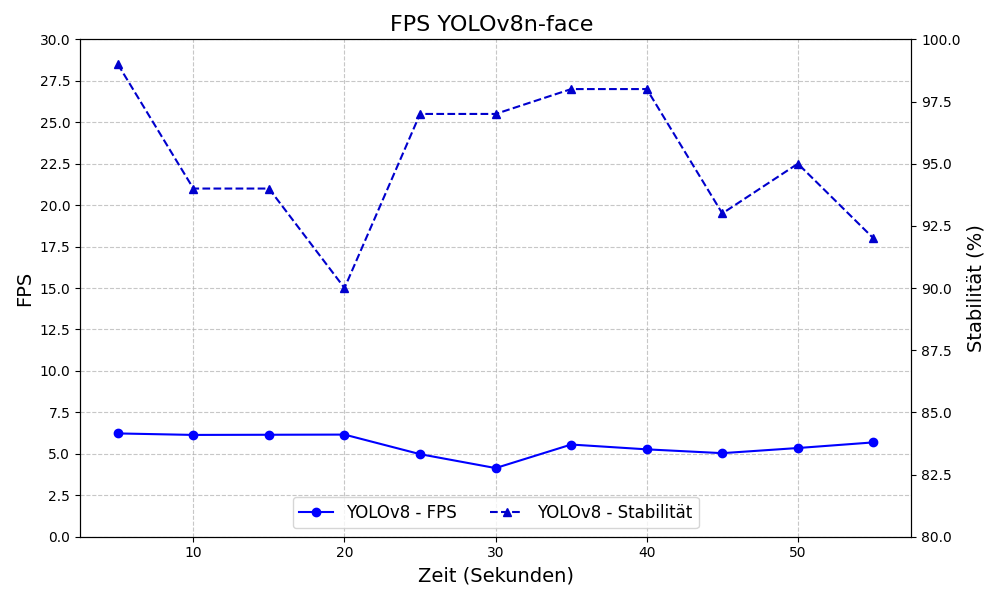
\includegraphics[width=\textwidth]{data/fps_yolo_detection.png}
        \caption{FPS und Stabilität YOLOv8-face}
        \label{fig:fps_yolo_detection}
    \end{subfigure}
    \begin{subfigure}{0.48\textwidth}
        \centering
        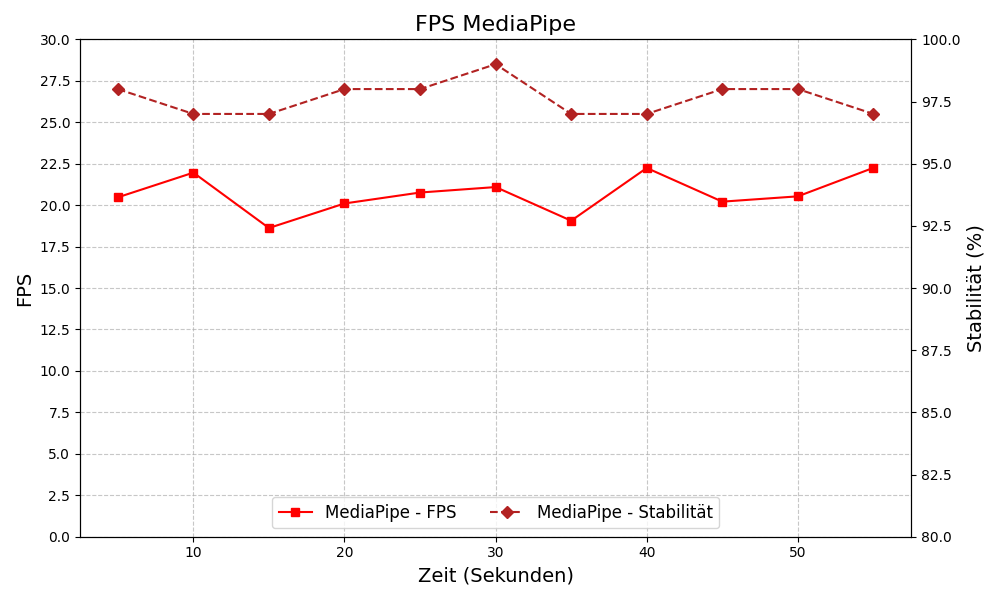
\includegraphics[width=\textwidth]{data/fps_mediapipe_detection.png}
        \caption{FPS und Stabilität MediaPipe FaceMesh}
        \label{fig:fps_mediapipe_detection}
    \end{subfigure}
    \caption{FPS und Stabilität der Gesichtserkennung mit YOLOv8-face und MediaPipe FaceMesh.}
    \label{fig:fps_comparison}
\end{figure}


\subsubsection{Projektdokumentation}

Im Rahmen des studentischen Projekts „Kennzeichen- und Gesichtserkennung mit YOLO" wurde ein technischer Demonstrator entwickelt, der als Lehrmaterial für zukünftige Studierende der THU Summer School konzipiert ist. Dieser Demonstrator ermöglicht mittels verschiedener Python-Bibliotheken wie ultralytics YOLO, mediapipe und tesseract die Erkennung sowohl von Fahrzeugkennzeichen als auch von menschlichen Gesichtern. Das sechsköpfige Team bestehend aus Chantal Deusch, Jeremy Diem, Jan Gaschler, Serhat Gürel, Paulina Pyczot und Valentin Talmon-L'Armée setzte das Projekt in einem Zeitraum von knapp zwei Monaten um, vom 12. März 2025 bis zum 4. Mai 2025.

Die Projektziele wurden zu Beginn in einem kooperativen Prozess mit dem Auftraggeber, Herrn Schäffter, definiert und hierarchisch strukturiert. Als primäre Ziele wurden sowohl funktionale als auch nicht-funktionale Anforderungen festgelegt. Auf funktionaler Ebene stand die Entwicklung eines benutzerfreundlichen Hands-On-Tutorials zur Inbetriebnahme von YOLO im Mittelpunkt, welches speziell für die THU Summer School konzipiert wurde. Dieses Tutorial sollte die Erkennung von Kennzeichen und Gesichtern unter kontrollierten Laborbedingungen ermöglichen und als Lehrmaterial von Studierenden für Studierende dienen. Die nicht-funktionalen Anforderungen beinhalteten eine kostengünstige Umsetzung, eine intuitive Benutzerfreundlichkeit sowie eine zuverlässige Funktionsweise des Systems.

Darüber hinaus wurden sekundäre Ziele definiert, welche die praktische Anwendbarkeit des Systems in realen Szenarien adressieren sollten. Im Bereich der Schrifterkennung wurde ein Anwendungsszenario für KFZ-Zutrittsschranken konzipiert, bei dem die Zuverlässigkeit unter verschiedenen Lichtverhältnissen eine besondere Herausforderung darstellte. Für die Personenerkennung wurde ein Zugangskontrollsystem für einen Supermarkt als exemplarisches Szenario entwickelt. Ein zusätzlicher Forschungsaspekt bestand in der kritischen Auseinandersetzung mit Sicherheitsrisiken durch die Exploration von Möglichkeiten zur Manipulation des eigenen Systems.

\paragraph{Vorgehensmodell und Teamstruktur}

\subparagraph{}{Vorgehensmodell}

Für die methodische Herangehensweise entschied sich das Projektteam für eine hybride Vorgehensweise, die Elemente aus SCRUM und Kanban kombinierte. Diese Entscheidung basierte auf der Notwendigkeit, sowohl eine strukturierte Planung als auch eine flexible Reaktion auf neue Erkenntnisse und Herausforderungen zu ermöglichen. In der Anfangsphase des Projekts wurde primär nach dem SCRUM-Rahmenwerk gearbeitet. Die Sprints wurden wöchentlich organisiert, wobei jeweils montags ein neuer Sprint begann und freitags mit einer Review abgeschlossen wurde. Das Sprint Planning für die kommende Woche erfolgte direkt im Anschluss an die Review am Freitag und wurde systematisch in Jira dokumentiert.

Mit fortschreitender Projektdauer, etwa ab Mitte April, zeigte sich jedoch, dass die strikte SCRUM-Methodik nicht optimal zur Dynamik des Projekts passte. Der administrative Aufwand für die SCRUM-Zeremonien band wertvolle Ressourcen, die für die technische Implementierung benötigt wurden. In einer gemeinsamen Entscheidung wurde daher ein Übergang zu einem Kanban-basierten Ansatz vollzogen. Diese Umstellung ermöglichte es dem Team, sich stärker auf die programmiertechnische Umsetzung zu konzentrieren und flexibler auf neue Erkenntnisse zu reagieren. Das Kanban-Board visualisierte den kontinuierlichen Arbeitsfluss und erleichterte die Priorisierung von Aufgaben ohne den Overhead formaler Sprint-Grenzen.

Diese adaptive Herangehensweise erwies sich als besonders vorteilhaft für ein Projekt mit einem hohen Anteil an experimenteller Arbeit und Programmieraufgaben. Die Kombination der strukturgebenden Elemente von SCRUM in der Initialisierungsphase mit der Flexibilität von Kanban in der Implementierungsphase trug wesentlich zum Projekterfolg bei.


%\begin{figure}[h]
%    \centering
%    % Hier würde ein Screenshot des Kanban Boards eingefügt werden
%    \caption{Kanban Board nach der Umstellung von SCRUM (Stand: 20.04.2025)}
%    \label{fig:kanban}
%\end{figure}

\subparagraph{}{Teamstruktur und Rollenverteilung}

Die Teamgröße von sechs Personen erwies sich als ideal für die funktionale Aufteilung in zwei Teilteams, die sich jeweils auf einen der Hauptaspekte des Projekts konzentrierten. Das erste Team, bestehend aus Jan Gaschler, Chantal Deusch und Paulina Pyczot, fokussierte sich auf die Entwicklung der Gesichtserkennungskomponente. Das zweite Team, mit den Mitgliedern Valentin Talmon-L'Armée, Serhat Gürel und Jeremy Diem, übernahm die Implementierung der Kennzeichenerkennung. Diese Aufteilung ermöglichte eine parallele Bearbeitung der beiden Hauptfunktionalitäten und förderte zugleich die Spezialisierung der Teammitglieder auf spezifische Technologien und Algorithmen.

Innerhalb der Gesamtstruktur wurden die klassischen SCRUM-Rollen definiert und besetzt: Paulina Pyczot übernahm die Rolle der Scrum Masterin und war somit für die Prozessoptimierung und die Beseitigung von Hindernissen verantwortlich. Valentin Talmon-L'Armée fungierte als Product Owner und vertrat die Interessen des Kunden im Team. Er priorisierte die Anforderungen und stellte sicher, dass das Produkt den Erwartungen des Auftraggebers entsprach. Alle Teammitglieder nahmen gleichzeitig die Rolle der Entwickler ein und waren aktiv an der technischen Implementierung beteiligt.

Diese Rollenverteilung schuf klare Verantwortlichkeiten und Kommunikationswege, während die funktionale Aufteilung in zwei Teilteams eine effiziente Parallelisierung der Arbeit ermöglichte. Die überschaubare Teamgröße begünstigte zudem einen engen Austausch und eine schnelle Entscheidungsfindung.

\subparagraph{}{Kommunikation und Arbeitsweise}

Die Kommunikation im Team erfolgte über verschiedene Kanäle, die je nach Kontext und Bedarf ausgewählt wurden. Discord diente als primäre Plattform für die interne Kommunikation, insbesondere für Daily Stand-ups, die schriftliche Protokollierung von Ergebnissen und die direkte Kommunikation mit den Betreuern. In spezifischen Discord-Channels wie „Schriftliches" und „Fragen an Betreuer" wurden To-Do-Listen und Meeting-Protokolle systematisch dokumentiert, um eine transparente Informationsbasis für alle Teammitglieder zu schaffen.

Microsoft Teams wurde vorrangig für die formellere Kommunikation genutzt, beispielsweise für Sprint Reviews, regelmäßige Statusberichte an Herrn Franz und den allgemeinen Austausch mit dem Kunden und den Betreuern. Zusätzlich diente Teams als zentrales Repository für wichtige Projektdokumente, die für alle Beteiligten zugänglich sein sollten.

Ergänzend zu den digitalen Kommunikationskanälen fanden regelmäßige Präsenztermine an der Hochschule statt. Im Projektraum wurden Jour Fixe-Termine mit dem Kunden und den Betreuern abgehalten, gemeinsame Programmier- und Brainstorming-Sessions durchgeführt sowie Retrospektiven und – vor der Umstellung auf Kanban – Sprint-Planungen organisiert. Diese Präsenztermine förderten den direkten Austausch und die Teambildung.

Die Arbeitsweise des Teams war durch verschiedene agile Praktiken geprägt. Daily Stand-ups wurden mittwochs und freitags in Präsenz durchgeführt, an den übrigen Tagen fanden sie online via Discord statt. Diese kurzen, fokussierten Meetings dienten dem Austausch über den aktuellen Fortschritt, bevorstehende Aufgaben und potenzielle Hindernisse. Die Durchführung erfolgte bedarfsorientiert, insbesondere wenn signifikante programmiertechnische Fortschritte erzielt wurden.

Zur kontinuierlichen Verbesserung der Zusammenarbeit wurden in regelmäßigen Abständen Retrospektiven durchgeführt. Dabei kamen verschiedene Methoden zum Einsatz, wie die „4L"-Methode (Liked, Learned, Lacked, Longed For, \cite{paula2025yolo}) oder der „Start-Stop-Continue"-Ansatz. Die Ergebnisse dieser Retrospektiven wurden auf virtuellen Whiteboards dokumentiert und bildeten die Grundlage für Prozessverbesserungen in den folgenden Projektphasen.

\begin{figure}[h]
    \centering
    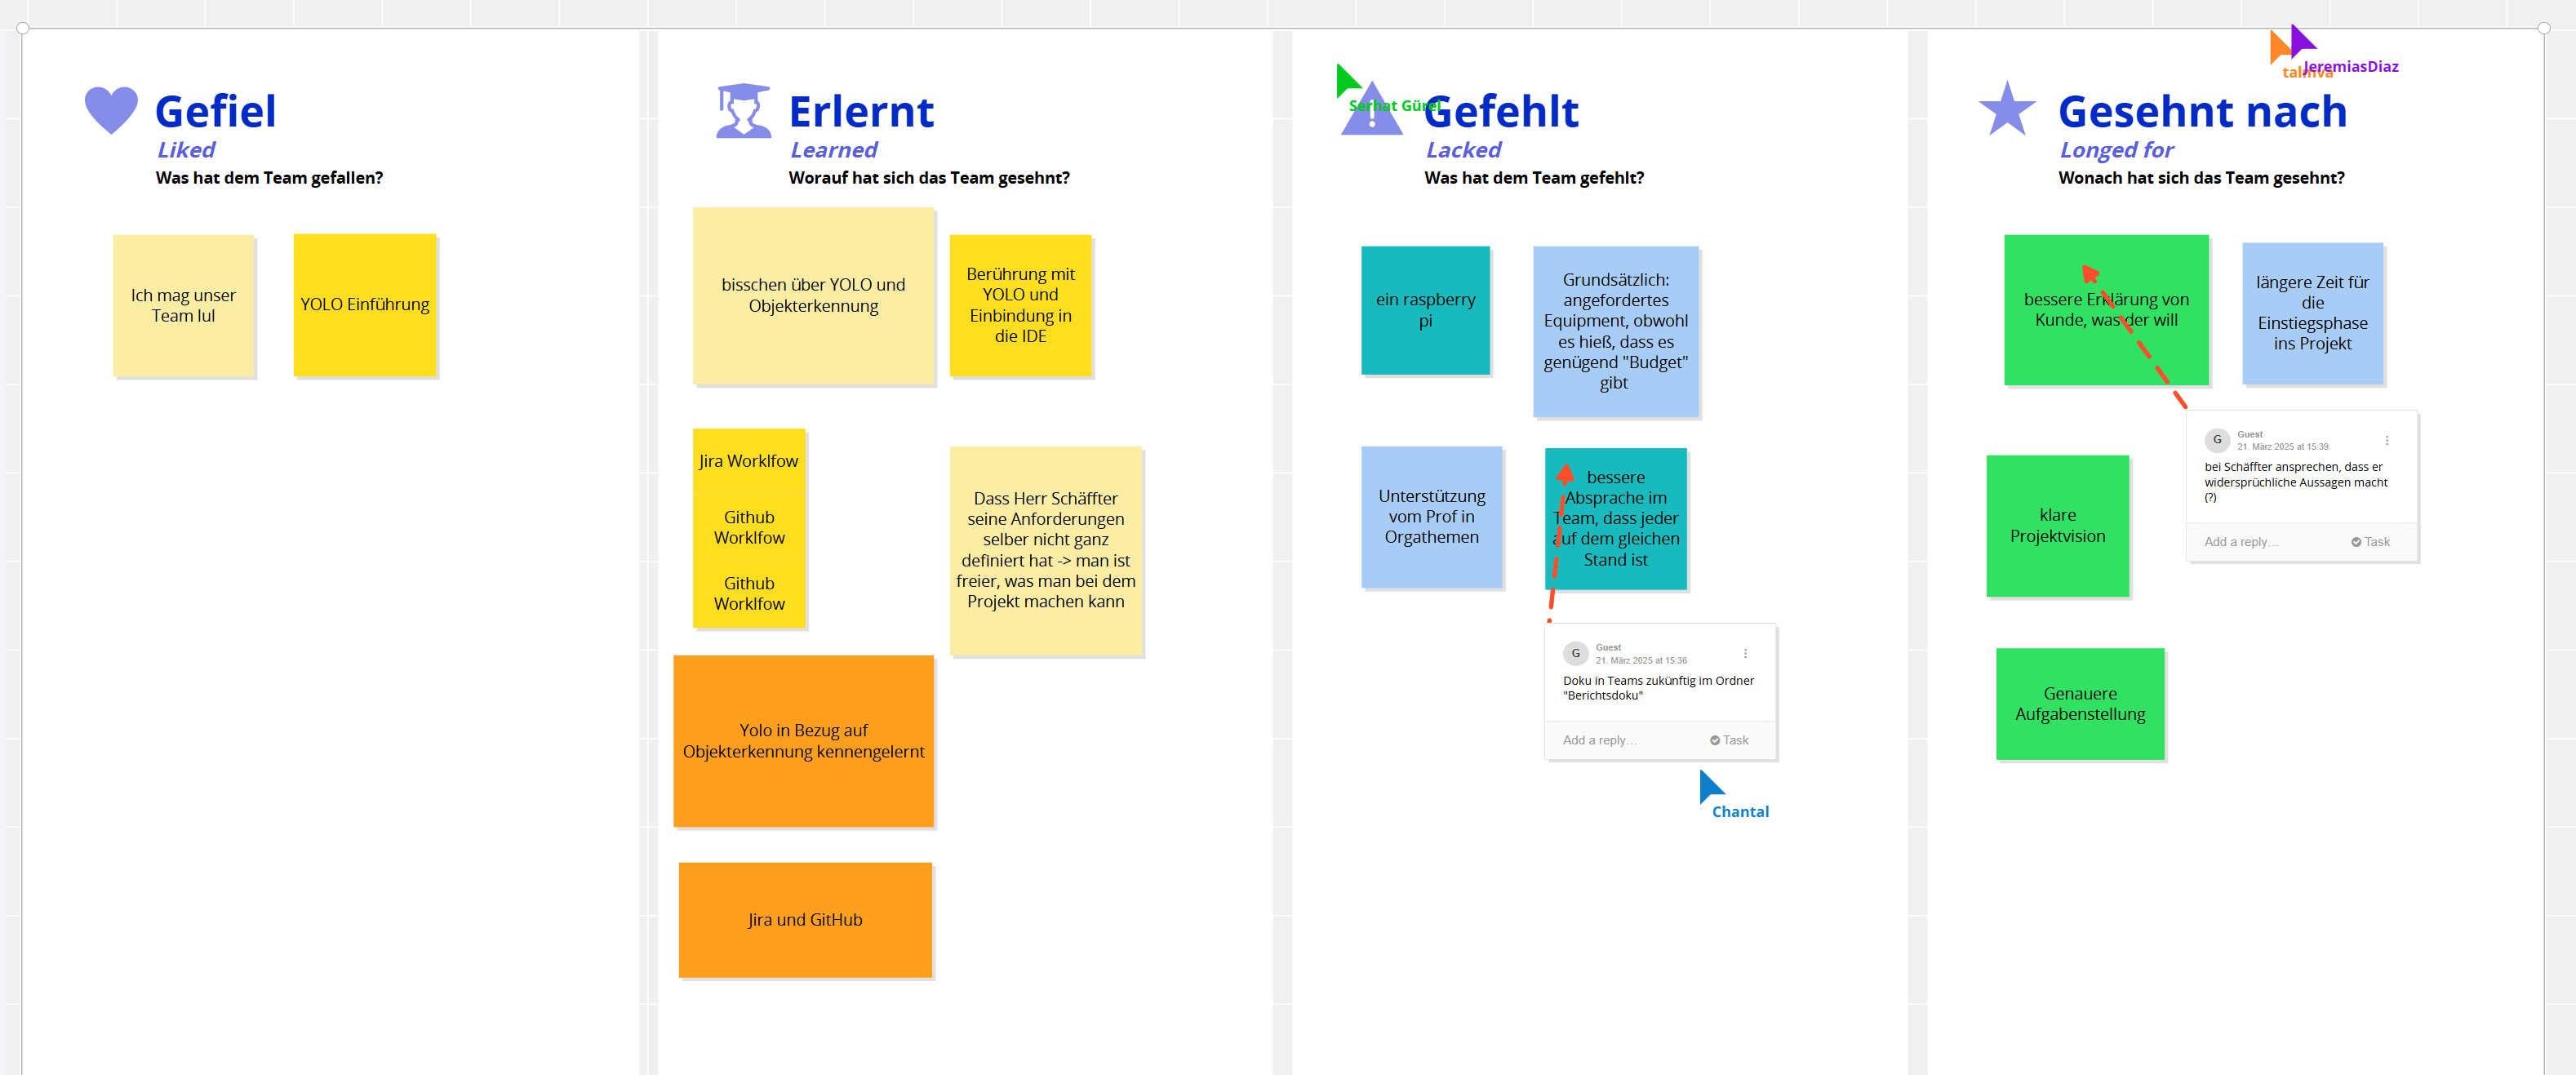
\includegraphics[width=1.0\textwidth]{data/4l.png}
    \caption{Retrospektive mit der 4L-Methode (durchgeführt am 21.03.2025)}
    \label{fig:da}
\end{figure}

Zu Beginn des Projekts wurde ein Backlog Refinement durchgeführt, um eine klare Priorisierung der Aufgaben zu etablieren und die Vision des Projekts zu schärfen. In der SCRUM-Phase wurden wöchentliche Sprints durchgeführt, die montags begannen und freitags endeten. Das Sprint Planning für den folgenden Sprint fand jeweils am Freitag statt und wurde detailliert in Jira dokumentiert, um eine strukturierte Übersicht über die anstehenden Aufgaben zu gewährleisten.

\paragraph{Dokumentation des Projektmanagements}

\subparagraph{}{Zeitplanung und Meilensteine}

Die Projektplanung basierte auf einem detaillierten Zeitplan, der die zentralen Meilensteine und Aktivitäten umfasste. Die chronologische Strukturierung des Projekts erfolgte entlang von acht wesentlichen Meilensteinen, die einen klaren Entwicklungspfad von der initialen Teamfindung bis zum Projektabschluss definierten.

Der erste Meilenstein umfasste die Phase der Teamfindung vom 6. Februar bis zum 10. März 2025, in der sich die sechs Teammitglieder zusammenfanden und erste konzeptionelle Überlegungen zum Projektumfang anstellten. Am 18. März 2025 wurde der zweite Meilenstein mit dem Abschluss der Projektplanung erreicht. In dieser Phase wurden die grundlegenden Strukturen für das Projektmanagement etabliert, Tools wie Jira und GitHub eingerichtet und erste inhaltliche Konzepte entwickelt.

Der dritte Meilenstein, die Implementierung der Kennzeichenerkennung unter Laborbedingungen, erstreckte sich vom 19. bis zum 27. März 2025. Hier lag der Fokus auf der Entwicklung eines grundlegenden Verständnisses der YOLO-Architektur und der Implementierung erster Erkennungsalgorithmen für Kennzeichen. Vom 28. März bis zum 3. April 2025 folgte der vierte Meilenstein mit der Erweiterung der Kennzeichenerkennung für das spezifische Anwendungsszenario an Mautstellen.

Der fünfte Meilenstein vom 4. bis zum 10. April 2025 widmete sich der Gesichtserkennung unter Laborbedingungen, gefolgt vom sechsten Meilenstein (11. bis 17. April 2025), der die Anwendung der Gesichtserkennung für Zutrittskontrollen adressierte. Der siebte Meilenstein vom 18. bis zum 25. April 2025 umfasste Untersuchungen zu Möglichkeiten der Manipulation von Gesichtserkennungssystemen und deren Absicherung.

Den Abschluss bildete der achte Meilenstein vom 26. April bis zum 2. Mai 2025, der die Präsentation des Projektergebnisses sowie die Finalisierung der Projektdokumentation beinhaltete. Diese strukturierte Zeitplanung ermöglichte eine kontinuierliche Fortschrittskontrolle und die frühzeitige Identifikation potenzieller Verzögerungen.

\begin{table}[h]
    \centering
    \begin{tabular}{|c|l|c|}
        \hline
        \textbf{Meilenstein} & \textbf{Beschreibung} & \textbf{Zeitraum} \\
        \hline
        1 & Teamfindung & 06.02.2025 - 10.03.2025 \\
        \hline
        2 & Projektplanung abgeschlossen & 18.03.2025 \\
        \hline
        3 & Kennzeichenerkennung unter Laborbedingungen & 19.03.2025 - 27.03.2025 \\
        \hline
        4 & Kennzeichenerkennung an Mautstellen & 28.03.2025 - 03.04.2025 \\
        \hline
        5 & Gesichtserkennung unter Laborbedingungen & 04.04.2025 - 10.04.2025 \\
        \hline
        6 & Gesichtserkennung für Zutrittskontrollen & 11.04.2025 - 17.04.2025 \\
        \hline
        7 & Manipulierte Gesichtserkennung & 18.04.2025 - 25.04.2025 \\
        \hline
        8 & Projektende mit Präsentation und Dokumentation & 26.04.2025 - 02.05.2025 \\
        \hline
    \end{tabular}
    \caption{Übersicht der Projektmeilensteine}
    \label{tab:milestones}
\end{table}

\subparagraph{}{Backlog-Management und Fortschrittskontrolle}

Das Backlog-Management wurde mithilfe von Jira realisiert, einer professionellen Software für agiles Projektmanagement. In Jira wurden sowohl das Product Backlog als auch die Sprint Backlogs systematisch gepflegt und kontinuierlich aktualisiert. In der SCRUM-Phase wurden regulär Burndown Charts erstellt, um den Fortschritt visuell zu erfassen und potenzielle Abweichungen vom geplanten Projektverlauf frühzeitig zu erkennen.

Insgesamt wurden über 90 Tickets im Jira-System erstellt und bearbeitet, die hierarchisch in acht Epic-Kategorien eingeordnet wurden, welche den definierten Meilensteinen entsprachen. Diese Struktur ermöglichte eine übersichtliche Organisation der anfallenden Aufgaben und erleichterte die Zuordnung von Verantwortlichkeiten.

Nach der Umstellung von SCRUM auf Kanban wurde das Jira-Board entsprechend angepasst, um den kontinuierlichen Arbeitsfluss transparent darzustellen. Anstelle der Sprint-gebundenen Planung trat nun die visualisierte Darstellung des Aufgabenflusses durch verschiedene Bearbeitungsstadien, was eine flexiblere Priorisierung und Bearbeitung der Aufgaben ermöglichte.

\begin{figure}[h]
    \centering
    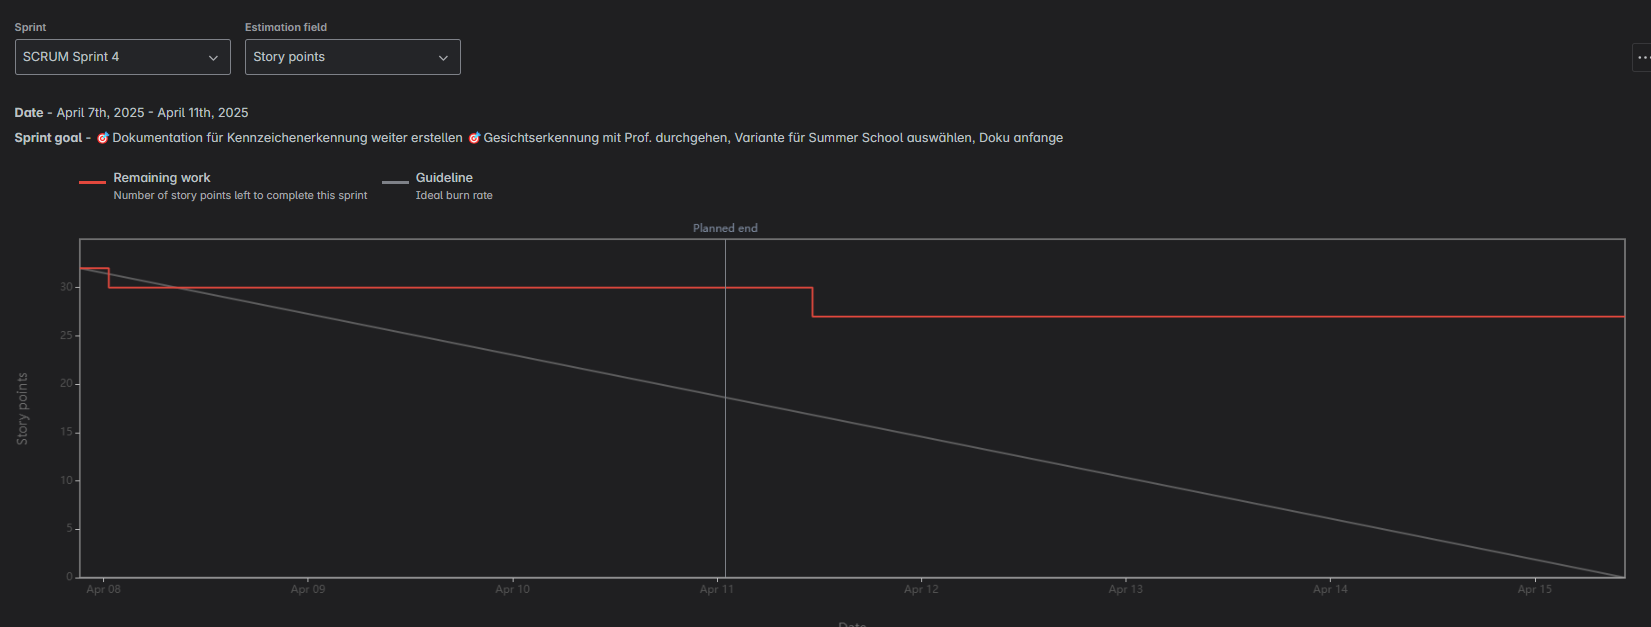
\includegraphics[width=1.0\textwidth]{data/burndown.png}
    \caption{Burndown Chart des letzten SCRUM-Sprints vor der Umstellung auf Kanban}
    \label{fig:burndown}
\end{figure}

Die Fortschrittskontrolle erfolgte durch regelmäßige Statusberichte, die an den Betreuer, Herrn Franz, übermittelt wurden. Diese Berichte boten eine konzise Zusammenfassung des aktuellen Projektstands, der erreichten Meilensteine und der geplanten nächsten Schritte. Ergänzend wurden Sprint-Review-Dokumente erstellt, die den Fortschritt bei der Implementierung der Kennzeichenerkennung und Gesichtserkennung detailliert dokumentierten.

Ein weiteres Element der Fortschrittskontrolle waren die Protokolle der regelmäßigen Meetings, die systematisch im Discord-Channel „Schriftliches" abgelegt wurden. Diese Protokolle dienten nicht nur der Dokumentation getroffener Entscheidungen, sondern auch als Basis für die Nachverfolgung von Aktionspunkten und offenen Fragen.

\subparagraph{}{Projektkommunikation und Dokumentationsmanagement}

Die Projektkommunikation erfolgte auf verschiedenen Ebenen und wurde durch eine strukturierte Dokumentation unterstützt. Während kein klassisches Lastenheft erstellt wurde, fanden regelmäßige Abstimmungen mit dem Kunden, Herrn Schäffter, statt, um den Projektumfang agil anzupassen. Ein Beispiel für diese agile Anpassungsfähigkeit war die Erweiterung des ursprünglich als „Personenerkennung mit YOLO" definierten Projekts um den Aspekt der Kennzeichenerkennung, um den Umfang besser an die zweimonatige Projektlaufzeit anzupassen.

To-Do-Listen wurden im Discord-Channel „Fragen an Betreuer" geführt und regelmäßig aktualisiert, um eine transparente Übersicht über anstehende Aufgaben zu gewährleisten. Diese Listen dienten als Ergänzung zum formalen Backlog in Jira und ermöglichten eine schnellere und direktere Kommunikation über kurzfristige Aufgaben.

Ein besonderer Fokus lag auf der Dokumentation der technischen Aspekte, insbesondere im Hinblick auf das zu erstellende Hands-On-Tutorial. Hier wurden detaillierte Anleitungen zur Einrichtung der Raspberry Pi-Umgebung, zur Installation der erforderlichen Bibliotheken und zur Nutzung der implementierten Erkennungsalgorithmen erstellt. Diese Dokumentation bildete die Grundlage für das Tutorial, das zukünftigen Studierenden der THU Summer School zur Verfügung gestellt werden sollte.

Im Bereich des Datenschutzes wurden potenzielle DSGVO-Implikationen frühzeitig mit Herrn Schäffter diskutiert, um sicherzustellen, dass die entwickelten Anwendungen den gesetzlichen Anforderungen entsprechen. Insbesondere für die Gesichtserkennung wurden Konzepte erarbeitet, die eine datenschutzkonforme Verarbeitung biometrischer Daten gewährleisteten.

\subparagraph{}{Versionsverwaltung und kollaboratives Arbeiten}

Für die Versionsverwaltung wurde GitHub als zentrales Repository genutzt. Um eine klare Trennung zwischen Entwicklung und Endprodukt zu gewährleisten, wurde das Projekt in zwei separate Repositories aufgeteilt: Ein privates Development-Repository für die Entwicklungsarbeit und ein öffentliches Repository für das Hands-on-Tutorial, das ohne direkten Zugriff auf die implementierten Lösungen genutzt werden konnte.

Die Branching-Strategie folgte einem strukturierten Ansatz, bei dem jedes Teammitglied auf einem eigenen Branch (\texttt{dev\_[Name]}) arbeitete. Diese dezentrale Arbeitsweise ermöglichte parallele Entwicklungen ohne gegenseitige Beeinträchtigungen. Funktionsfähiger Code wurde auf den \texttt{development}-Branch zusammengeführt, wobei die Integration erst nach erfolgreichen Tests erfolgte. Nur vollständig fertiggestellte und getestete Funktionen wurden mittels Pull Request auf den \texttt{main}-Branch übertragen, der stets eine stabile und produktionsreife Version des Projekts repräsentierte.

Für Pull Requests wurde eine standardisierte Checkliste implementiert, die eine konsistente Qualitätssicherung gewährleistete. Diese Checkliste umfasste unter anderem die detaillierte Beschreibung der Änderung, die Kategorisierung der Art der Änderung (neue Funktion, Bugfix, Breaking Change, Dokumentationsupdate), eine Auflistung der durchgeführten Tests, die Bestätigung der Einhaltung der Stilrichtlinien, den Nachweis eines Self-Reviews, die Kommentierung komplexer Codeabschnitte, die Anpassung der zugehörigen Dokumentation, die Vermeidung neuer Warnungen, das Hinzufügen von Tests für neue Funktionen sowie die erfolgreiche lokale Ausführung aller Tests. Diese umfassende Checkliste stellte sicher, dass nur qualitativ hochwertiger und gut dokumentierter Code in das Hauptrepository integriert wurde.

Das kollaborative Arbeiten wurde durch diese strukturierte Versionsverwaltung erheblich erleichtert. Die klare Trennung der Arbeitsbereiche durch individuelle Branches verhinderte Konflikte bei der gleichzeitigen Bearbeitung von Dateien, während die zentralisierte Integration über den \texttt{development}-Branch eine kontinuierliche Integration der Einzelbeiträge zu einem kohärenten Gesamtsystem ermöglichte.

\subparagraph{}{Reflexion und Verbesserungspotential}

Die Entscheidung, von SCRUM zu Kanban zu wechseln, erwies sich im Projektverlauf als vorteilhaft und angemessen. Die anfängliche SCRUM-Struktur bot einen soliden Rahmen für die Projektinitialisierung und -planung, während Kanban in der Umsetzungsphase die erforderliche Flexibilität bereitstellte. Diese Anpassungsfähigkeit war besonders wertvoll angesichts des experimentellen Charakters des Projekts und der Tatsache, dass alle Teammitglieder parallel zu ihren regulären Studienverpflichtungen am Projekt arbeiteten.

In der Retrospektive lassen sich dennoch verschiedene Bereiche identifizieren, in denen Verbesserungspotential bestand. Eine präzisere Einschätzung des Arbeitsaufwands zu Beginn des Projekts hätte möglicherweise zu einer realistischeren Zeitplanung geführt und damit einige der zeitlichen Herausforderungen in den späteren Projektphasen reduziert. Die anfängliche Planung erwies sich teilweise als zu optimistisch, insbesondere hinsichtlich der Komplexität der Implementierung der Gesichtserkennung.

Der Wechsel zu Kanban hätte eventuell früher erfolgen können, da der administrative Aufwand für die SCRUM-Methodik teilweise Ressourcen band, die für die technische Umsetzung hätten genutzt werden können. Eine frühere Erkenntnis der besseren Eignung des Kanban-Ansatzes für dieses spezifische Projekt hätte möglicherweise zu einer effizienteren Ressourcennutzung geführt.

Die Dokumentation der technischen Aspekte erfolgte teilweise erst gegen Projektende, was den Abschlussprozess intensivierte. Eine kontinuierlichere Dokumentation parallel zur Entwicklung hätte eine gleichmäßigere Arbeitsbelastung ermöglicht und potenziell zu einer höheren Dokumentationsqualität geführt. Zudem hätte eine intensivere Testphase, insbesondere für die Überprüfung des Hands-On-Tutorials durch unbeteiligte Dritte, möglicherweise weitere Verbesserungspotentiale aufgedeckt.

Trotz dieser Optimierungsmöglichkeiten kann das Projektmanagement insgesamt als erfolgreich betrachtet werden. Die flexible Kombination aus SCRUM und Kanban ermöglichte es dem Team, die auftretenden Herausforderungen zu bewältigen und die primären Projektziele zu erreichen. Die klare Strukturierung in Meilensteine, die transparente Kommunikation und die systematische Versionsverwaltung trugen wesentlich zum Gelingen des Projekts bei. Die entwickelten Erkennungsalgorithmen für Kennzeichen und Gesichter sowie das erstellte Hands-On-Tutorial erfüllen die anfangs definierten Anforderungen und bieten eine solide Grundlage für zukünftige Weiterentwicklungen und Anwendungen im Rahmen der THU Summer School.